\documentclass[10pt,a4paper]{article}
\usepackage[utf8]{inputenc}
\usepackage[spanish]{babel}
\usepackage{amsmath}
\usepackage[colorlinks=true, linkcolor=black, urlcolor=blue]{hyperref}
\usepackage{amsfonts}
\usepackage{amssymb}
\usepackage{float}
\usepackage{tabularx}
\usepackage{graphicx}
\usepackage[usenames,dvipsnames]{color}
\usepackage{lmodern}
\usepackage[left=2cm,right=2cm,top=2cm,bottom=2cm]{geometry}
\usepackage{color}%para poder definir, utilizar colores en fuente, fondo...etc
\setcounter{page}{0}%Para que la página de título no se tenga en cuenta
\usepackage{natbib}
\usepackage{hyperref}
\usepackage{eurosym}
\setcounter{secnumdepth}{5} %Para subsubsusbsection, se debe poner paragraph.

\usepackage{listings}%Entornos de código
\usepackage{color}

\definecolor{mygreen}{rgb}{0,0.6,0}
\definecolor{gray}{rgb}{0.5,0.5,0.5}
\definecolor{mauve}{rgb}{0.58,0,0.82}

%\lstset{frame=tb,
%  language=Java,
%  aboveskip=3mm,
%  belowskip=3mm,
%  showstringspaces=false,
%  columns=flexible,
%  basicstyle={\small\ttfamily},
%  numberstyle=\tiny\color{gray},
%  keywordstyle=\color{blue},
%  commentstyle=\color{dkgreen},
%  stringstyle=\color{mauve},
%  breaklines=true,
%  breakatwhitespace=true
%  tabsize=2
%}

\lstset{frame=tb,
  language=Java,% Set your language (you can change the language for each code-block optionally)
  basicstyle=\footnotesize\ttfamily,
  numbers=left,
  morekeywords={end},
  aboveskip=3mm,
  belowskip=3mm,
  backgroundcolor=\color{white},
  frame=single,
  showstringspaces=false,
  columns=flexible,
  basicstyle={\small\ttfamily},
  numberstyle=\tiny\color{gray},
  keywordstyle=\color{mauve},
  commentstyle=\color{mygreen},
  stringstyle=\color{blue},
  breaklines=true,
  breakatwhitespace=true,
  tabsize=2
}

\setlength{\parskip}{2mm}%Separación entre párrafos.

%kuggle.com  


\author{Jose Ignacio Sánchez\\Josu Rodríguez}
\title{\begin{center}\textbf{\Huge{Minería de datos} Práctica 1:Clustering knn-means}
%\begin{center}\includegraphics[scale=0.5]{./img/SVM-classifiers.jpg} 
%\footnote{Imagen
%extraida de \url{http://www.thebookmyproject.com/cars/intrusion-detection-technique-using-k-means-fuzzy-neural-network-svm-classifiers/intrusion-detection-technique-by-using-k-means-fuzzy-neural-network-and-svm-classifiers/}}
%\end{center} 
\end{center}}
\date{\today}


\newtheorem{defi}{(\it Definición)}[section]%Para obtener las definiciones enumeradas, con la sección que las contiene
\newtheorem{teorema}{(\it Teorema)}[section]%Para obtener los teoremas enumeradas, con la sección que las contiene

\makeindex

\renewcommand{\tablename}{\textbf{Tabla}}

\begin{document}

\maketitle

\thispagestyle{empty}%para evitar enumeración de la página de la portada y del índice

\newpage

%Tabla de contenido
\renewcommand\contentsname{\centering ÍNDICE DE CONTENIDO}
\tableofcontents%índice
\thispagestyle{empty}
\newpage

%Lista de tablas
\renewcommand{\listtablename}{\centering ÍNDICE DE TABLAS} %Para cambiar el índice de las tablas
\listoftables
\thispagestyle{empty}
\newpage

%lista de figuras 
\renewcommand\listfigurename{\centering ÍNDICE DE FIGURAS}
\thispagestyle{empty}
\listoffigures
\clearpage

\setcounter{page}{1}%Para reinizar el contador de páginas en la página deseada

\section{Introducción}

El objetivo principal de esta práctica es obtener la capacidad de formular un
algoritmo de aprendizaje automático de clasificación \textbf{\textit{No-Supervisada}}. 
Por otra parte, se trabajarán la capacidad de sintetizar uns técnica de aprendizaje automático
no-supervisado, conocer su coste computacional así como sus limitaciones de representación
y de inteligibilidad \par

%\begin{defi}
%	Esto es una definición o teorema.
%\end{defi}

\section{Recursos}
\begin{itemize}
	\item PC con aplicación Weka.
	\item Bibliografía.
	\item Librerías de  Weka.
	\item Manual de Weka.
	\item Guía de la práctica.
	\item Ficheros para los datos de la
	práctica:
	\textcolor{green}{food.arff},
	\textcolor{green}{colon.arff}.
	\item Otros ficheros que no están en formato \textit{.arff}:
		\begin{itemize}
			\item En formato \textit{.txt}: \textcolor{green}{ClusterData.atributos.txt} (este fichero si tiene la clase asociada para 
			evaluar la calidad del \textit{clustering} en \textcolor{green}{ClusterData.clase.txt}).
			\item E formato \textit{.csv} \textcolor{green}{bank-data.csv}clustering
		\end{itemize}
\end{itemize}

\section{Clasificación \textbf{NO-supervisada} o \textit{Clustering}}

\begin{defi}
	Se considera \textbf{clasificación no-supervisada} cuando el conjunto de
	entrenamiento  no están las instancias etiquetadas con el valor de la clase. Es
	un experimento exploratorio, que trata de agrupar las instancias en grupos
	definidos por similitud entre las características de las instancias que
	pertenecen al mismo grupo y disimilitud entre las que pertenecen a grupos
	distintos. Tecnicamente estos grupos son llamados \textit{Clusters}.
\end{defi}

\subsection{Clustering \textit{\textbf{k-means}}}


\section{Diseño}
 
 Estructuramos la ejecución del algoritmo en fases\ref{fig:dependencias} , las cuales se definen a continuación.\\
 
\subsection*{Primera fase: carga de datos y configuración}
 
 Inicialmente se encarga de cargar el fichero en una estructura de datos adecuada para el cálculo del algoritmo.Además se carga la configuración establecida
 por el usuario, es decir que tipo de inicialización para el \textit{codebook}, número de clusters, distancia a utilizar\dots

\subsection*{Segunda fase: Preproceso de datos}

En el preproceso se normaliza el espacio, haciendo uso de la función estadística zscore, es decir a cada \textit{Feature} de la instancia se le resta su media y dividiendo el resultado por la varianza de dicha \textit{Feature} se consigue que todos los valores de los atributos se encuentren dentro del intervalo [-1,1]. Con ésto conseguimos evitar la mayor influencia de algunos atributos debido a que se encuentren dentro de un dominio de valores mayor. Por ejemplo si vamos a agrupar viviendas y utilizamos como características el número de habitaciones y el precio, seguramente el número de habitaciones no será mucho mayor de 3 y en cambio el precio puede ser mayor incluso de 300000 \euro .\cite{coursera}

\subsection*{Tercera Fase: Algoritmo K-means}

En esta fase se implementa el algoritmo \textbf{K-means}.
\begin{enumerate}
	\item En primer lugar inicia los \textit{centroides} con el criterio establecido por el usuario, o la matriz de bits de pertenencias.
	\item Recorre las instancias del conjunto y calcula la distancia a cada uno de los \textit{codeword} actualizando la matriz de bits de pertenencia,el valor 		del bit es uno si es el centroide más cercano a la instancia.
	\item Se calcula de nuevo el vector promedio para cada cluster.
	\item Iterar los pasos dos y tres hasta converger.
\end{enumerate}

\subsection*{Cuarta Fase: Evaluación}

En esta fase se tratará de automatizar la evaluación del algoritmo frente a los datos obtenidos con distintas ejecuciones, variando los parámetros o incluso con  
los resultados obtenidos con el modelo de \textbf{K-means} que ya implementa el API de \textbf{weka}.

\subsection*{Dependencias}
 %mapa de diseño donde se muestran las dependencias y se documentan las rutinas.
\begin{figure}[h!]
	\centering
	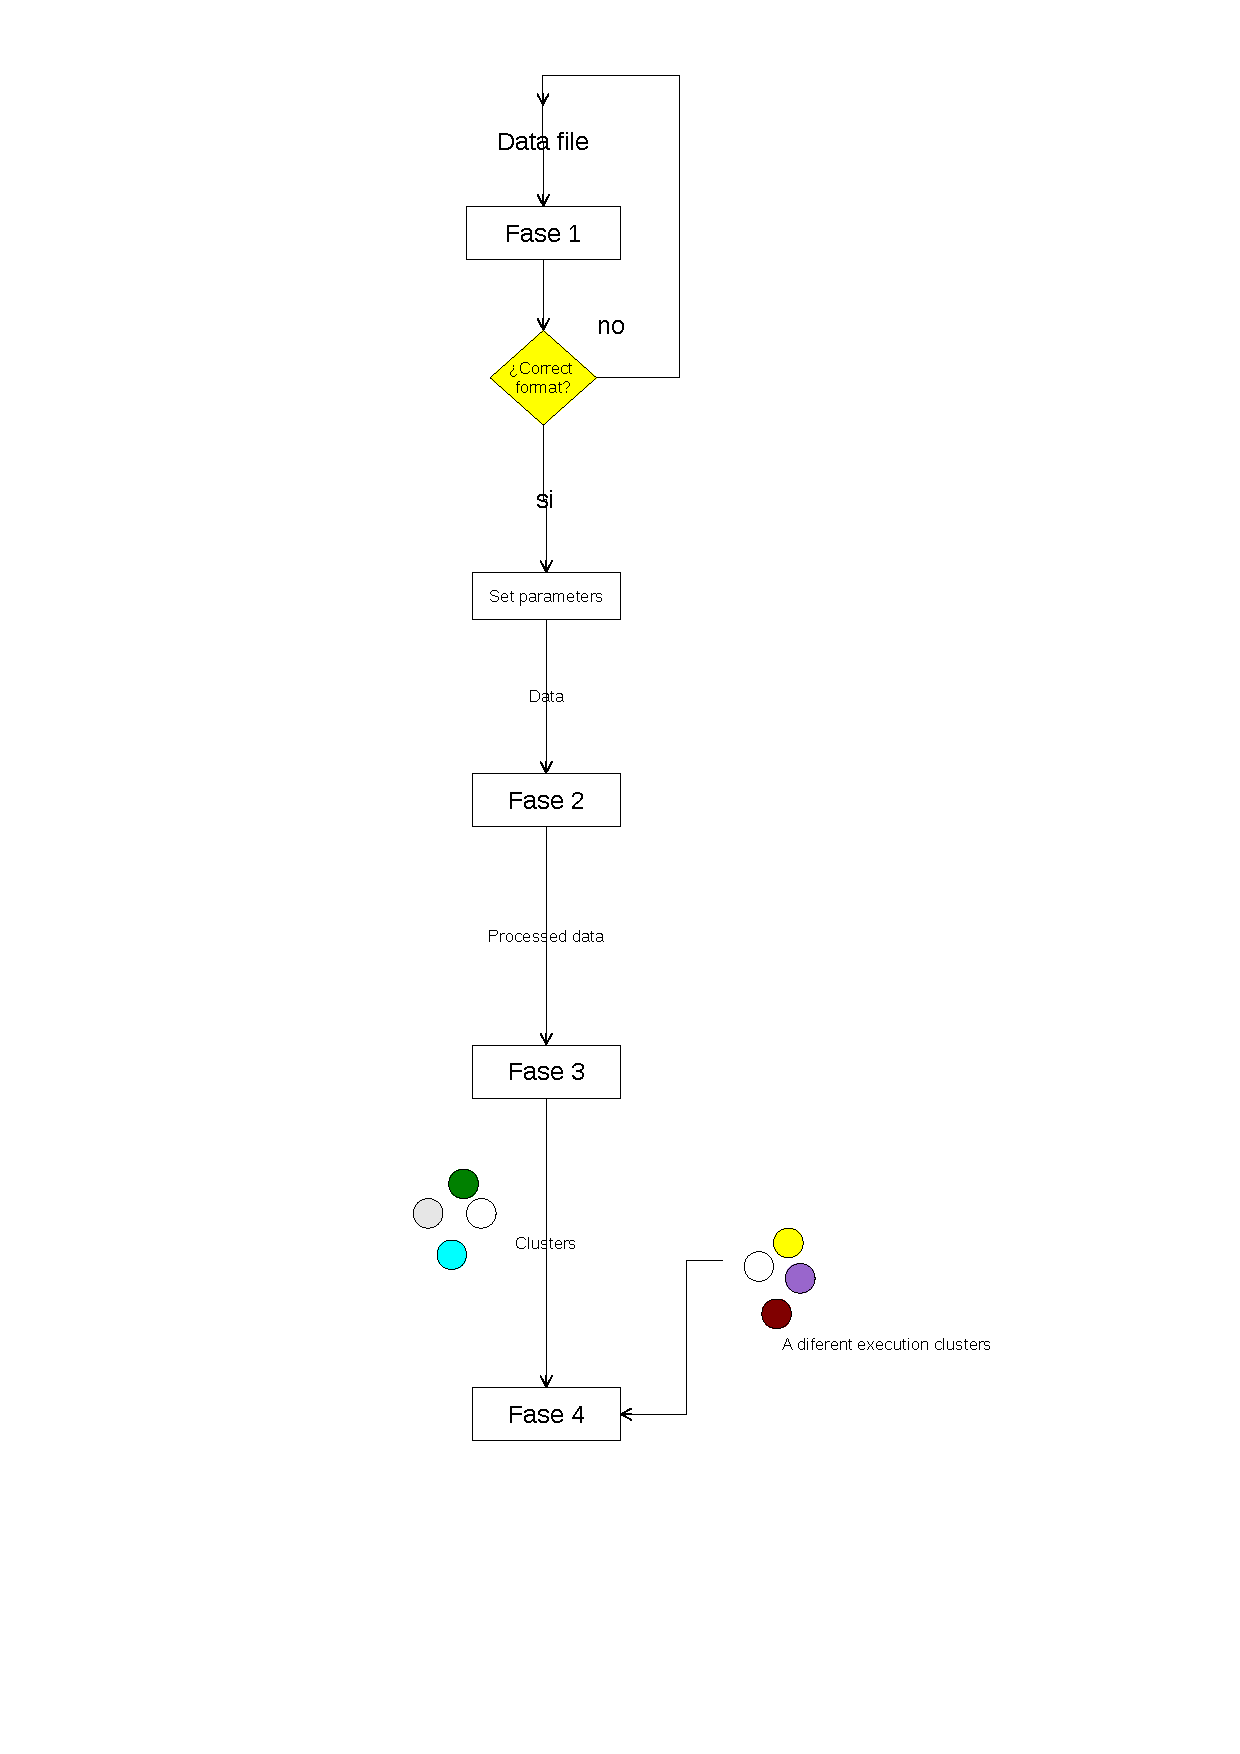
\includegraphics[scale=0.50]{./img/dependenciasKmeans.pdf}%crear esquema para incluirlo
	\caption[Esquema de dependencias del sistema]{Dependencias del sistema}
	\label{fig:dependencias}
\end{figure}

%\footnotetext{Imagen obtenida de:
%\href{http://stackoverflow.com/questions/6160495/support-vector-machines-a-simple-explanation}{http://stackoverflow.com/questions/6160495/support-vector-machines-a-simple-explanation}.}

%\footnotetext{Imagen obtenida de:
%\href{http://en.wikipedia.org/wiki/File:Svm\_max\_sep\_hyperplane\_with\_margin.png}{\nolinkurl{http://en.wikipedia.org/wiki/File:Svm\_max\_sep\_hyperplane\_with\_margin.png}}.}

%\begin{equation}
%	min\frac{1}{2}||w||^{2}
%	\label{eq:pl}
%\end{equation}

\subsection{Algoritmo en pseudocódigo}

\begin{lstlisting}
Let k be the number of clusters to partition the data set
Let X = {x1,x2, ..., xn} be the data set to be analyzed
Let M = {m1, m2, ..., mk} be the code-book associated to the clusters
Let dist(a, b) be the desired distance metric
Let B = {B11, B12, ..., Bnk} be the temporary pertenece bit matrix

Ensure: C = {C1, C2, ..., CK} set of clusterized instances

Begin:

	for each mj
		mj = randomsample(X)
	end
		
	for each xn
		Cj = argmin dist (xi,mj) // para cada j, como la formulita del armgin de siempre. en vez del igual tengo que mirar algo que simbolice a�adir
	end
		
	while changes in M do
		for each mj
			mjnew = calculatecentroid(Cj)
			if mjnew == mj
				changes = false
			else
				changes = true
			end
			mj = mjnew	
		end
		
		for each xn
			// Cj = argmin dist (xi,mj) // lo mismo que arriba, mirar� a hacerlo con f�rmulas de latex despu�s de que lo repases posibilidad 1, sin matriz de pertenencia
			
			Bnj = 1 sii argmin dist (xn,mj) = mj (para cada mj) si no Bnj = 0 
		end
		
		for each Bij 
			if Bij == 1
				Cj = xi (a�adir xi a Cj)
			end
		end
	end
	
	return C = {C1, C2, ..., Ck}
end
\end{lstlisting}
\section{Implementación}

\subsubsection{Problemas encontrados} 

\subsubsection{Soluciones adoptadas} 

\section{Validación del \textit{software}}

\subsection{Diseño del banco de pruebas}

\section{Análisis de resultados}

\subsection{Modificando inicializaciones}

\subsection{Modificando distancia Minkowski}

\subsection{Criterios de convergencia}

\subsubsection{Número fijo de iteraciones}

\subsubsection{Disimilitud entre \textit{codebooks}}

\subsection{Distintas métricas}

\subsubsection{Manhattan}

\subsubsection{Euclídea}

\subsubsection{Minkowski}

\section{Clasificación supervisada respecto de }

%\section{Preproceso de los datos}
%
%\subsubsection{Randomize}
%
%\subsubsection{Normalize}
%
%\subsubsection{Outliers y Extreme Values}
%
%\subsubsection{Problemas al implementar el preproceso de datos}
%
%\subsection{Utils}
%
%\subsubsection{StopWatch}
%
%Esta función se encarga de indicarnos el tiempo transcurrido, en segundos,
%desde donde se instancia el objeto, hasta donde se para el
%contador\par
%
%Creemos necesario su uso, ya que nos aporta una visión objetiva del coste de tiempo computacional 
%de los distintos algoritmos implementados,como por ejemplo en el proceso de
%clasificación de las instancias sin estimar incluidas en los distintos conjuntos de
%test.
%
%\subsubsection{VerboseCutter}
%
%Esta MAE se encarga de eliminar la salida de sistema que
%imprime al hacer la evaluación el clasificador \textit{LibSVM} por defecto.\par
%
%La implementación de esta funcionalidad ha sido posible gracias a la inestimable
%ayuda por parte de otro de los grupos\footnote{David Ramírez, Begoña Carcedo,
%Andoni Martín, Marta Aguilera}.\par
%
%Eliminando la salida de sistema, podemos mostrar de forma más
%clara infomación relevante de nuestro programa, facilitando, de esta manera,
%la comprensión de los datos por parte del usuario.Además se puede seguir
%revisando dicha salida en el fichero temporal al que ha sido redireccionada.\par
%
%\paragraph{Problemas de ejecución:}
%	Al activar y desactivar esta MAE dentro de bucles anidados, no obtenemos el
%	resultado deseado, esto ocurre por falta de capacidad de respuesta por
%	capacidad de procesamiento y velocidad de escritura/lectura del disco.
%\paragraph{Solución:}
%	Aunque con desactivar la salida antes de cada evaluación es suficiente, hemos
%	sacado la llamada a la MAE fuera de los bucles(antes de los bucles se desactiva y despues de los bucles se activa la salida de sistema).
%	De esta manera hemos conseguido los resultados deseados.



\section{Conclusiones}

	\begin{itemize}
		\item Breve descripción de las motivaciones para llevar a cabo técnicas de clustering.
		\item Conclusiones a la vista de los resultados más relevantes.
		\item Conclusiones generales.(Análisis de fortalezas del sw y reflexiones sobre la tarea.
		\item Análisis de puntos débiles y propuestas de mejoras.
	\end{itemize}

\section{Valoración subjetiva}

\begin{enumerate}

	\item ¿Has alcanzado los objetivos que se plantean? 
	
	\item ¿Te ha resultado de utilidad la tarea planteada?

	\item ¿Qué dificultades has encontrado?Valora el grado de dificultad de la tarea.

	\item  ¿Cuánto tiempo has trabajado en esta tarea? Desglosado:

		\begin{table}[H]
		\centering
		\resizebox{8cm}{!}{
						\begin{tabular}{|l|l|}
							\hline
							\multicolumn{2}{|c|}{\textbf{Coste temporal}}\\
							\hline
								Diseño de software & \\
								Implementación de software & \\
								Tiempo trabajando con Weka & \\
								Búsqueda bibliográfica & \\
								Informe & 1\\
								\hline
							\end{tabular}
						}
		\end{table}

	\item  Sugerencias para mejorar la tarea. Sugerencias para que se consiga
	despertar mayor interés y motivación en los alumnos.\par

	\item  Críticas(constructivas).

\end{enumerate} 

\newpage

\bibliographystyle{plain}
\bibliography{bibliografia}

%Ser crítico, analizar datos experemientales.Aplicar pequeños heurísticos.

\end{document} 
